\documentclass[12pt,a4paper]{article}

% ─── Page Layout ───────────────────────────────────────────────────────────────
\usepackage[a4paper, margin=0.8in, headheight=14pt]{geometry}

% ─── Fonts (XeLaTeX) ───────────────────────────────────────────────────────────
\usepackage{fontspec}
\usepackage{unicode-math}
\setmainfont{TeX Gyre Pagella}
\setmonofont[Scale=0.88]{TeX Gyre Cursor}
\setmathfont{Latin Modern Math}

% ─── Packages ──────────────────────────────────────────────────────────────────
\usepackage{xcolor}
\usepackage{colortbl}
\usepackage{titlesec}
\usepackage{enumitem}
\usepackage{tabularx}
\usepackage{longtable}
\usepackage{booktabs}
\usepackage{array}
\usepackage{amsmath}
\usepackage{tikz}
\usetikzlibrary{shapes.geometric, arrows.meta, positioning, calc, fit, decorations.pathreplacing, patterns}
\usepackage{tcolorbox}
\tcbuselibrary{skins, breakable}
\usepackage{hyperref}
\usepackage{fancyhdr}
\usepackage{graphicx}
\usepackage{microtype}
\hyphenpenalty=10000
\exhyphenpenalty=10000
\sloppy
\usepackage{caption}
\usepackage{setspace}
\usepackage{multirow}
\usepackage{tocloft}

% ─── Q&A helper ────────────────────────────────────────────────────────────────
\newcommand{\Q}[1]{\textbf{#1}\par\noindent\ignorespaces}

% ─── Colour Palette ────────────────────────────────────────────────────────────
\definecolor{myred}{RGB}{196,30,58}
\definecolor{mydark}{RGB}{30,30,50}
\definecolor{mygreen}{RGB}{14,120,80}
\definecolor{myteal}{RGB}{0,130,140}
\definecolor{myamber}{RGB}{180,100,0}
\definecolor{mypurple}{RGB}{100,30,160}
\definecolor{mygray}{RGB}{246,247,249}
\definecolor{mgframe}{RGB}{180,185,200}
\definecolor{watermark}{RGB}{145,150,170}
\definecolor{hdrred}{RGB}{250,232,235}
\definecolor{hdrgreen}{RGB}{220,244,233}
\definecolor{hdrteal}{RGB}{220,242,244}
\definecolor{hdramber}{RGB}{253,242,215}
\definecolor{hdrpurple}{RGB}{238,228,255}
\definecolor{hdrgray}{RGB}{238,240,245}

% ─── Section Formatting ────────────────────────────────────────────────────────
\titleformat{\section}
  {\large\bfseries\color{myred}}{\thesection.}{0.5em}{}
  [\vspace{1pt}{\color{myred}\rule{\linewidth}{0.8pt}}]
\titleformat{\subsection}
  {\normalsize\bfseries\color{myteal}}{\thesubsection}{0.5em}{}
\titlespacing*{\section}{0pt}{18pt}{7pt}
\titlespacing*{\subsection}{0pt}{11pt}{4pt}

% ─── Paragraph ─────────────────────────────────────────────────────────────────
\setlength{\parindent}{0pt}
\setlength{\parskip}{4pt}

% ─── TOC Styling ───────────────────────────────────────────────────────────────
\renewcommand{\cfttoctitlefont}{\large\bfseries\color{myred}}
\renewcommand{\cftaftertoctitle}{\par\noindent{\color{myred}\rule{\linewidth}{0.8pt}}}
\setlength{\cftbeforetoctitleskip}{0pt}
\setlength{\cftaftertoctitleskip}{6pt}
\renewcommand{\cftsecfont}{\normalsize\bfseries\color{mydark}}
\renewcommand{\cftsecpagefont}{\normalsize\bfseries\color{mydark}}
\renewcommand{\cftsecleader}{\cftdotfill{\cftdotsep}}
\setlength{\cftbeforesecskip}{7pt}
\renewcommand{\cftsubsecfont}{\small\color{mydark}}
\renewcommand{\cftsubsecpagefont}{\small\color{mydark}}
\setlength{\cftbeforesubsecskip}{3pt}
\setlength{\cftsubsecindent}{1.4em}

% ─── Table helpers ─────────────────────────────────────────────────────────────
\renewcommand{\arraystretch}{1.45}
\setlength{\tabcolsep}{6pt}
\arrayrulecolor{mydark}
\newcolumntype{B}[1]{>{\small\bfseries\raggedright\arraybackslash}m{#1}}
\newcolumntype{Y}{>{\small\raggedright\arraybackslash}X}
\renewcommand{\tabularxcolumn}[1]{m{#1}}

% ─── Header / Footer ───────────────────────────────────────────────────────────
\pagestyle{fancy}
\fancyhf{}
\fancyhead[L]{\small\color{myred}\textbf{EC403}\;\color{mydark}--- Microprocessor and Microcontroller}
\fancyhead[R]{\small\color{myteal}\textbf{Module 4 Notes}}
\fancyfoot[C]{\small\color{mydark}\thepage}
\fancyfoot[R]{\small\color{watermark}\textit{\copyright\ Biraj Sarkar (CGEC)}}
\renewcommand{\headrulewidth}{0.5pt}
\renewcommand{\footrulewidth}{0.3pt}

% ─── Hyperref ──────────────────────────────────────────────────────────────────
\hypersetup{
  colorlinks=true, linkcolor=myteal, urlcolor=myteal,
  pdfauthor={Biraj Sarkar (CGEC)},
  pdftitle={EC403 --- Module 4 Notes: RISC Processors and ARM Microcontroller Interface Design}
}

% ─── tcolorbox styles ──────────────────────────────────────────────────────────
\tcbset{
  tikzbox/.style={
    colback=mygray, colframe=mgframe, boxrule=0.6pt, arc=4pt,
    left=8pt, right=8pt, top=6pt, bottom=6pt,
    colbacktitle=mgframe, coltitle=mydark, fonttitle=\small\bfseries
  },
  defbox/.style={
    colback=hdrgreen, colframe=mygreen, boxrule=0.8pt, arc=4pt,
    left=9pt, right=9pt, top=6pt, bottom=6pt,
    colbacktitle=mygreen, coltitle=white, fonttitle=\small\bfseries
  },
  formulabox/.style={
    colback=hdrteal, colframe=myteal, boxrule=0.8pt, arc=4pt,
    left=9pt, right=9pt, top=7pt, bottom=7pt,
    colbacktitle=myteal, coltitle=white, fonttitle=\small\bfseries
  },
  examplebox/.style={
    colback=hdramber, colframe=myamber, boxrule=0.8pt, arc=4pt,
    left=9pt, right=9pt, top=6pt, bottom=6pt,
    colbacktitle=myamber, coltitle=white, fonttitle=\small\bfseries
  },
  masonbox/.style={
    colback=hdrpurple, colframe=mypurple, boxrule=0.8pt, arc=4pt,
    left=9pt, right=9pt, top=6pt, bottom=6pt,
    colbacktitle=mypurple, coltitle=white, fonttitle=\small\bfseries
  },
  exambox/.style={
    colback=hdrpurple, colframe=mypurple, boxrule=1pt, arc=5pt,
    left=10pt, right=10pt, top=8pt, bottom=8pt,
    colbacktitle=mypurple, coltitle=white, fonttitle=\bfseries,
    breakable, title after break={\textbf{Frequently Asked / Viva Questions (contd.)}}
  }
}
\tcbset{breakable}
\tcbset{after={\par\color{black}}}

% ─── TikZ styles ───────────────────────────────────────────────────────────────
\tikzset{
  block/.style={rectangle, draw=myteal, fill=hdrteal,
    text width=2.4cm, align=center, minimum height=0.95cm,
    font=\small, rounded corners=3pt, line width=0.7pt},
  redblock/.style={rectangle, draw=myred, fill=hdrred,
    text width=2.4cm, align=center, minimum height=0.95cm,
    font=\small, rounded corners=3pt, line width=0.7pt},
  amberblock/.style={rectangle, draw=myamber, fill=hdramber,
    text width=2.4cm, align=center, minimum height=0.95cm,
    font=\small, rounded corners=3pt, line width=0.7pt},
  sumjunc/.style={circle, draw=myamber, fill=hdramber,
    minimum size=0.62cm, font=\small, line width=0.8pt},
  arrow/.style={-Stealth, thick, color=mydark},
  redarrow/.style={-Stealth, thick, color=myred},
  line/.style={thick, color=mydark}
}

\begin{document}

% ─── Title Page ───────────────────────────────────────────────────────────────
\begin{center}
  {\LARGE\bfseries\color{myred} EC403 --- Microprocessor and Microcontroller}\\[5pt]
  {\normalsize\color{mydark} Semester IV \quad$\bullet$\quad 3L:0T:0P \quad$\bullet$\quad 3 Credits}\\[3pt]
  {\normalsize\color{myteal}\textbf{Module 4 Exam Notes: RISC Processors and ARM Interface Design}}\\[3pt]
  {\small\color{mydark} CGEC \;$|$\; B.Tech ECE (2023--27) \;$|$\; \textit{Biraj Sarkar}}
\end{center}
\vspace{2pt}
\noindent{\color{myred}\rule{\linewidth}{1.5pt}}
\vspace{2pt}

\hypersetup{linkcolor=mydark}
\tableofcontents
\hypersetup{linkcolor=myteal}
\newpage

\section{Introduction to RISC Processors}

\begin{tcolorbox}[defbox, title={RISC vs. CISC Design Philosophy}]
A \textbf{Reduced Instruction Set Computer (RISC)} is a processor architecture designed around a small, highly optimized set of simple, uniform-length instructions that execute in a single clock cycle through deep pipelining and hardwired control logic.

In contrast, a \textbf{Complex Instruction Set Computer (CISC)} provides a vast, heterogeneous library of variable-length instructions capable of performing multi-step operations (e.g., memory-to-memory arithmetic) using microprogrammed control memory and variable execution cycles.
\end{tcolorbox}

\subsection{CISC vs. RISC Comprehensive Comparison}
\par\vspace{6pt}
\begingroup
\setlength{\extrarowheight}{2.5pt}
\setlength{\LTleft}{0pt}
\setlength{\LTright}{0pt}
\begin{longtable}{|B{3.2cm}|>{\small\raggedright\arraybackslash}m{\dimexpr(\linewidth-3.2cm-6\tabcolsep-4\arrayrulewidth)/2\relax}|>{\small\raggedright\arraybackslash}m{\dimexpr(\linewidth-3.2cm-6\tabcolsep-4\arrayrulewidth)/2\relax}|}
\hline
\textbf{Parameter} & \textbf{CISC (e.g., Intel x86, 8085)} & \textbf{RISC (e.g., ARM, MIPS, RISC-V)} \\ \hline
\endfirsthead
\hline
\textbf{Parameter} & \textbf{CISC (e.g., Intel x86, 8085)} & \textbf{RISC (e.g., ARM, MIPS, RISC-V)} \\ \hline
\endhead
Instruction Length & Variable ($1$ to $15$ bytes in x86). & Fixed uniform length (strictly $32$ bits; $16$-bit in Thumb). \\ \hline
Instruction Execution & Multi-cycle execution ($1$ to $50+$ cycles). & Single-cycle execution per instruction stage ($CPI \approx 1$). \\ \hline
Memory Operations & Arithmetic/logic directly accesses memory operands (`ADD [BX], AX`). & Strict \textbf{Load/Store Architecture}: memory access only via `LDR`/`STR`; arithmetic is register-to-register. \\ \hline
Addressing Modes & Numerous, complex modes ($10+$ modes). & Few, simple, orthogonal addressing modes ($2$ to $4$ modes). \\ \hline
Register File & Small, specialized register sets (e.g., $AX, BX, CX, DX, SP, BP$). & Large, uniform, orthogonal general-purpose register file ($32+$ registers). \\ \hline
Control Unit & Microprogrammed control store (ROM based, complex sequencer). & Fast \textbf{Hardwired Control Logic} (combinational logic gates and PLAs). \\ \hline
Pipelining & Difficult due to variable instruction lengths and multi-cycle execution. & Highly efficient, uniform, predictable instruction pipelining. \\ \hline
Compiler Design & Simpler compiler; complex silicon hardware. & Optimizing compiler bears complexity to schedule instructions and pipeline slots. \\ \hline
\end{longtable}
\endgroup

\section{RISC Pipelining and Pipeline Hazards}

\subsection{The Classic 5-Stage RISC Pipeline}
A classic RISC processor partitions instruction execution into 5 discrete, balanced stages:
\begin{enumerate}[leftmargin=*]
  \item \textbf{IF (Instruction Fetch):} Fetches the 32-bit instruction word from Instruction Memory using the Program Counter ($\mathrm{PC}$); updates $\mathrm{PC} \leftarrow \mathrm{PC} + 4$.
  \item \textbf{ID (Instruction Decode \& Register Read):} Decodes the opcode and reads operand values from the dual-read-port register file.
  \item \textbf{EX (Execute / Address Calculation):} Performs arithmetic/logical operations via the ALU or calculates the memory effective address.
  \item \textbf{MEM (Memory Access):} Performs data memory read (`LDR`) or data memory write (`STR`). For non-memory instructions, this stage is a pipeline bypass.
  \item \textbf{WB (Write Back):} Writes the computation or loaded memory result back into the destination register in the register file.
\end{enumerate}

\begin{tcolorbox}[tikzbox, title={Execution Flow Across 5-Stage RISC Pipeline}]
\centering
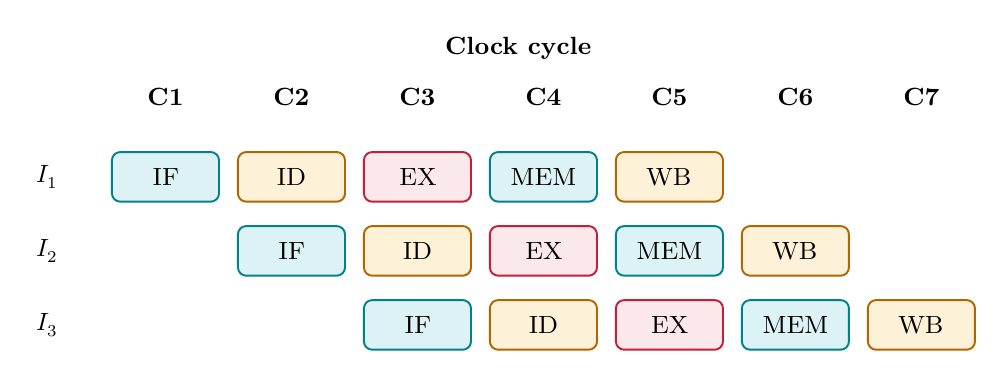
\begin{tikzpicture}[x=1.6cm,y=0.94cm,every node/.style={font=\small},
  stage/.style={align=center,text width=1.12cm,minimum width=1.36cm,minimum height=0.63cm,inner sep=2pt}]
  \node[font=\small\bfseries] at (3.3,1.74) {Clock cycle};
  \foreach \cycle in {1,...,7}
    \node[font=\small\bfseries] at (\cycle-0.5,1.08) {C\cycle};

  \foreach \instruction in {1,...,3} {
    \node[anchor=east] at (-0.27,1-\instruction) {$I_{\instruction}$};
    \node[block,stage] at (\instruction-0.5,1-\instruction) {IF};
    \node[amberblock,stage] at (\instruction+0.5,1-\instruction) {ID};
    \node[redblock,stage] at (\instruction+1.5,1-\instruction) {EX};
    \node[block,stage] at (\instruction+2.5,1-\instruction) {MEM};
    \node[amberblock,stage] at (\instruction+3.5,1-\instruction) {WB};
  }
\end{tikzpicture}
\end{tcolorbox}

\subsection{Pipeline Performance and Speedup}
For a $k$-stage pipeline executing $n$ independent instructions:
\begin{itemize}[leftmargin=*]
  \item Non-pipelined execution time: $T_{\mathrm{non-pipe}} = n \times k \times \tau$.
  \item Pipelined execution time: $T_{\mathrm{pipe}} = [k + (n - 1)] \times \tau$.
  \item \textbf{Theoretical Pipeline Speedup ($S_k$):}
  \[
  \mathbf{S_k} = \frac{T_{\mathrm{non-pipe}}}{T_{\mathrm{pipe}}} = \frac{n \times k}{k + n - 1} \xrightarrow{n \to \infty} \mathbf{k}
  \]
  An ideal $5$-stage pipeline delivers a theoretical speedup of $5\times$ over non-pipelined execution.
\end{itemize}

\subsection{Pipeline Hazards and Resolution Strategies}
A pipeline hazard is any condition that prevents the next instruction in the instruction stream from executing during its designated clock cycle:
\begin{enumerate}[leftmargin=*]
  \item \textbf{Structural Hazards (Resource Conflicts):}
  \begin{itemize}[leftmargin=*]
    \item Occur when two separate pipeline stages attempt to access the identical hardware unit simultaneously (e.g., IF reading instruction while MEM writes data into a single unified memory).
    \item \textbf{Resolution:} Adopt \textbf{Harvard Architecture} with separate physical Instruction and Data memories/caches.
  \end{itemize}
  \item \textbf{Data Hazards (Data Dependencies):}
  \begin{itemize}[leftmargin=*]
    \item Occur when an instruction depends on the result of a prior in-flight instruction that has not yet completed execution.
    \item \textbf{Read-After-Write (RAW, True Dependency):} $I_2$ reads a register before $I_1$ writes it.
    \item \textbf{Write-After-Read (WAR, Anti-Dependency):} $I_2$ attempts to write before $I_1$ reads.
    \item \textbf{Write-After-Write (WAW, Output Dependency):} $I_2$ attempts to write before $I_1$ writes.
    \item \textbf{Resolution Strategies:}
    \begin{itemize}[leftmargin=*]
      \item \textbf{Operand Forwarding (Bypassing):} Routes intermediate calculation results directly from the EX/MEM or MEM/WB pipeline registers to the ALU input multiplexer, bypassing the register file and eliminating stalls.
      \item \textbf{Load-Delay Slot / Stalling:} A `LDR` instruction produces data only after the MEM stage; an immediate dependent instruction must be stalled by 1 cycle (bubble) or scheduled with an independent instruction by the compiler.
    \end{itemize}
  \end{itemize}
  \item \textbf{Control Hazards (Branch Penalties):}
  \begin{itemize}[leftmargin=*]
    \item Occur when branch or jump instructions alter sequential program flow, invalidating instructions already fetched into the pipeline.
    \item \textbf{Branch Penalty:} Stalls the pipeline for $(k-1)$ cycles if resolved late.
    \item \textbf{Resolution:} Delayed branching (filling the branch delay slot with an independent useful instruction), static branch prediction, or dynamic branch prediction using a 2-bit Branch Target Buffer (BTB).
  \end{itemize}
\end{enumerate}

\begin{tcolorbox}[tikzbox, title={Hardware Operand Forwarding (Bypass) Mechanism}]
\centering
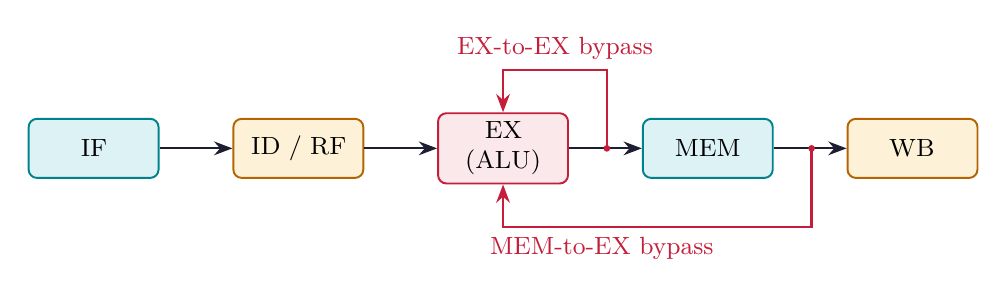
\begin{tikzpicture}[every node/.style={font=\small},
  stage/.style={align=center,text width=1.38cm,minimum width=1.65cm,minimum height=0.75cm,inner sep=3pt}]
  \node[block,stage] (fetch) at (0,0) {IF};
  \node[amberblock,stage] (decode) at (2.6,0) {ID / RF};
  \node[redblock,stage] (ex) at (5.2,0) {EX (ALU)};
  \node[block,stage] (mem) at (7.8,0) {MEM};
  \node[amberblock,stage] (wb) at (10.4,0) {WB};

  \draw[arrow,thick] (fetch.east) -- (decode.west);
  \draw[arrow,thick] (decode.east) -- (ex.west);
  \draw[arrow,thick] (ex.east) -- (mem.west);
  \draw[arrow,thick] (mem.east) -- (wb.west);

  \coordinate (exout) at ($(ex.east)!0.52!(mem.west)$);
  \coordinate (memout) at ($(mem.east)!0.52!(wb.west)$);
  \draw[redarrow,thick] (exout) -- ++(0,1.0) -|
    node[pos=0.25,above] {EX-to-EX bypass} (ex.north);
  \draw[redarrow,thick] (memout) -- ++(0,-1.0) -|
    node[pos=0.34,below] {MEM-to-EX bypass} (ex.south);
  \fill[myred] (exout) circle[radius=1.2pt] (memout) circle[radius=1.2pt];
\end{tikzpicture}
\end{tcolorbox}

\section{ARM Core Architecture and Programmer's Model}

\begin{tcolorbox}[defbox, title={ARM Architecture Overview}]
\textbf{ARM (Advanced RISC Machines)} is a family of 32-bit RISC processor cores licensed by ARM Holdings. Key architectural hallmarks include:
\begin{itemize}[leftmargin=*]
  \item Strict 32-bit Load/Store architecture.
  \item Orthogonal, uniform 32-bit instruction format.
  \item Dedicated hardware \textbf{Barrel Shifter} attached to ALU operand path.
  \item \textbf{Conditional execution} available on all 32-bit instructions.
  \item Compact 16-bit \textbf{Thumb instruction set} for high code density.
\end{itemize}
\end{tcolorbox}

\subsection{ARM7TDMI Core Specifications}
The \textbf{ARM7TDMI} core is the classic 32-bit workhorse of embedded systems:
\begin{itemize}[leftmargin=*]
  \item \textbf{T (Thumb):} Supports the 16-bit Thumb instruction set, achieving up to $35\%$ code density reduction while executing on a 16-bit external memory bus.
  \item \textbf{D (Debug):} On-chip JTAG debug interface for hardware breakpoints and register inspection.
  \item \textbf{M (Multiplier):} Enhanced 32-bit hardware multiplier yielding $32 \times 32$ and $64$-bit results in few clock cycles.
  \item \textbf{I (EmbeddedICE):} Integrated on-chip hardware in-circuit emulator logic for real-time debugging.
  \item \textbf{Pipeline:} 3-stage pipeline (Fetch, Decode, Execute).
\end{itemize}

\begin{tcolorbox}[tikzbox, title={ARM Core Datapath: Inline Barrel Shifter and ALU}]
\centering
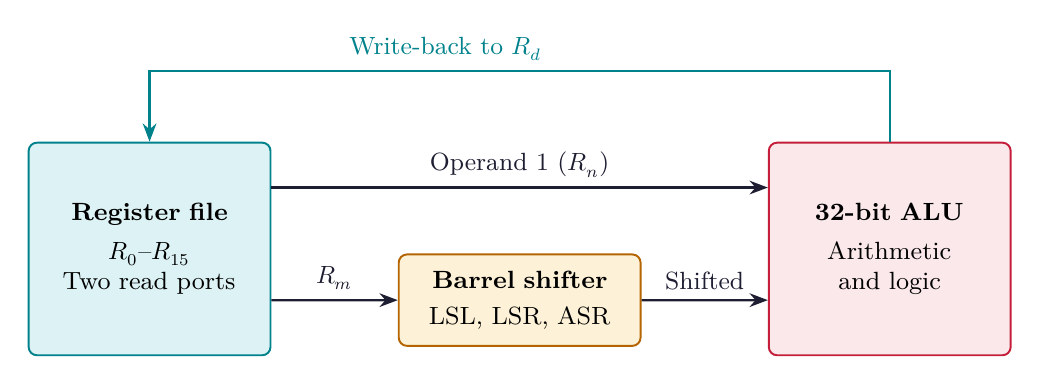
\begin{tikzpicture}[every node/.style={font=\small},
  unit/.style={align=center,text width=2.65cm,inner sep=6pt}]
  \node[block,unit,minimum height=2.7cm] (rf) at (0,0)
    {\textbf{Register file}\\[3pt] $R_0$--$R_{15}$\\ Two read ports};
  \node[amberblock,unit] (shift) at (4.7,-0.65)
    {\textbf{Barrel shifter}\\[2pt] LSL, LSR, ASR};
  \node[redblock,unit,minimum height=2.7cm] (alu) at (9.4,0)
    {\textbf{32-bit ALU}\\[3pt] Arithmetic and logic};

  \draw[arrow,thick] ([yshift=0.78cm]rf.east) --
    node[above] {Operand 1 ($R_n$)} ([yshift=0.78cm]alu.west);
  \draw[arrow,thick] ([yshift=-0.65cm]rf.east) --
    node[above] {$R_m$} (shift.west);
  \draw[arrow,thick] (shift.east) --
    node[above] {Shifted} ([yshift=-0.65cm]alu.west);
  \draw[arrow,thick,myteal] (alu.north) -- ++(0,0.9) -|
    node[pos=0.30,above] {Write-back to $R_d$} (rf.north);
\end{tikzpicture}
\end{tcolorbox}

\subsection{ARM Cortex-M Series Architecture}
The \textbf{ARM Cortex-M} family is optimized for deeply embedded microcontroller applications:
\par\vspace{6pt}\noindent
\begingroup
\setlength{\extrarowheight}{2.5pt}
\begingroup
\setlength{\LTleft}{0pt}
\setlength{\LTright}{0pt}
\begin{longtable}{|B{2.6cm}|B{2.2cm}|B{3.2cm}|>{\small\raggedright\arraybackslash}m{\dimexpr(\linewidth-2.6cm-2.2cm-3.2cm-8\tabcolsep-5\arrayrulewidth)/1\relax}|}
\hline
\textbf{Core} & \textbf{Instruction Set} & \textbf{Pipeline Depth} & \textbf{Key Target Applications} \\ \hline
\endfirsthead
\hline
\textbf{Core} & \textbf{Instruction Set} & \textbf{Pipeline Depth} & \textbf{Key Target Applications} \\ \hline
\endhead
Cortex-M0 / M0+ & Thumb / Thumb-2 subset & 2 or 3 stages & Ultra-low power 8-bit/16-bit microcontroller replacements, smart sensors. \\ \hline
Cortex-M3 & Full Thumb-2 (32/16-bit) & 3 stages with branch speculation & Standard 32-bit microcontrollers (e.g., STM32F103), automotive, industrial control. \\ \hline
Cortex-M4 & Thumb-2 + DSP + FPU & 3 stages & Motor control, digital signal processing, audio, power conversion. \\ \hline
Cortex-M7 & Thumb-2 + Double FPU & 6 stages (Dual-issue superscalar) & High-performance embedded computing, advanced graphics, robotics. \\ \hline
\end{longtable}
\endgroup\par
\endgroup

\subsection{Nested Vectored Interrupt Controller (NVIC)}
The \textbf{NVIC} is a tightly integrated hardware interrupt controller built into all Cortex-M cores:
\begin{itemize}[leftmargin=*]
  \item \textbf{Deterministic Low Latency:} Extremely fast interrupt entry (e.g., strictly 12 clock cycles on Cortex-M3).
  \item \textbf{Automatic Hardware Stacking:} Core registers ($R_0-R_3, R_{12}, LR, PC, xPSR$) are automatically pushed onto the active stack by hardware on interrupt entry and popped upon return.
  \item \textbf{Tail-Chaining:} When an interrupt arrives while executing another ISR, the processor skips the pop/push stack cycle, switching to the new ISR in only 6 clock cycles.
  \item \textbf{Late-Arriving Handling:} If a higher-priority interrupt arrives while stacking for a lower-priority interrupt, the NVIC immediately switches to the higher-priority vector without restarting stacking.
\end{itemize}

\begin{tcolorbox}[tikzbox, title={NVIC Low-Latency Tail-Chaining Mechanism}]
\centering
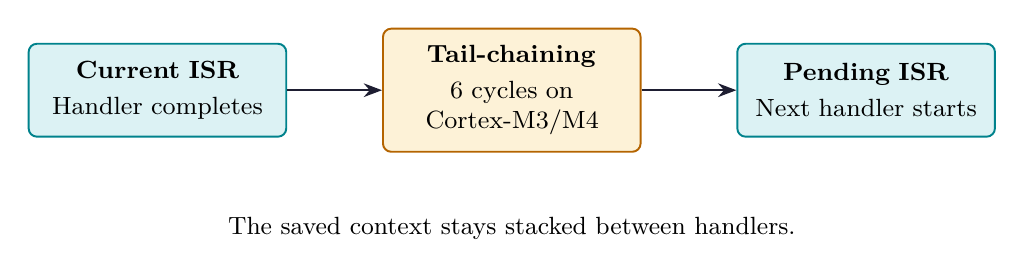
\begin{tikzpicture}[every node/.style={font=\small},
  unit/.style={align=center,text width=2.85cm,minimum height=1.18cm,inner sep=6pt}]
  \node[block,unit] (first) at (0,0) {\textbf{Current ISR}\\[2pt] Handler completes};
  \node[amberblock,unit] (chain) at (4.5,0) {\textbf{Tail-chaining}\\[2pt] 6 cycles on Cortex-M3/M4};
  \node[block,unit] (second) at (9.0,0) {\textbf{Pending ISR}\\[2pt] Next handler starts};
  \draw[arrow,thick] (first.east) -- (chain.west);
  \draw[arrow,thick] (chain.east) -- (second.west);
  \node[below=7mm of chain,align=center]
    {The saved context stays stacked between handlers.};
\end{tikzpicture}
\end{tcolorbox}

\subsection{ARM Programmer's Model: Registers and Status Flags}
An ARM core provides 16 visible 32-bit core data registers and Program Status Registers:
\begin{itemize}[leftmargin=*]
  \item \textbf{$R_0$ to $R_{12}$:} General-Purpose Registers for operands and addresses.
  \item \textbf{$R_{13}$ (Stack Pointer, SP):} In Cortex-M, physically implemented as two banked registers:
  \begin{itemize}[leftmargin=*]
    \item \textbf{MSP (Main Stack Pointer):} Used by OS kernel and exception/interrupt handlers.
    \item \textbf{PSP (Process Stack Pointer):} Used by application user tasks in an RTOS.
  \end{itemize}
  \item \textbf{$R_{14}$ (Link Register, LR):} Holds the subroutine return address upon executing a `BL` (Branch with Link) instruction; holds \texttt{EXC\_RETURN} codes during interrupts.
  \item \textbf{$R_{15}$ (Program Counter, PC):} Holds the address of the currently executing instruction plus pipeline offset ($+8$ bytes in ARM state due to 3-stage pipeline).
  \item \textbf{Current Program Status Register (CPSR / xPSR):}
  \par\vspace{4pt}
  \centering
  \begin{tabular}{|c|c|c|c|c|c|c|c|c|c|}
  \hline
  \textbf{$D_{31}$} & \textbf{$D_{30}$} & \textbf{$D_{29}$} & \textbf{$D_{28}$} & \textbf{$D_{27}$} & $\cdots$ & \textbf{$D_7$} & \textbf{$D_6$} & \textbf{$D_5$} & \textbf{$D_{4}-D_0$} \\ \hline
  \textbf{N} & \textbf{Z} & \textbf{C} & \textbf{V} & \textbf{Q} & $\cdots$ & \textbf{I} & \textbf{F} & \textbf{T} & \textbf{Mode} \\ \hline
  \end{tabular}
  \par\vspace{4pt}\raggedright
  \begin{itemize}[leftmargin=*, itemsep=2pt]
    \item \textbf{N (Negative):} Set if bit 31 of result is 1; \textbf{Z (Zero):} Set if result is 0.
    \item \textbf{C (Carry):} Set on arithmetic carry / borrow; \textbf{V (Overflow):} Set on signed overflow.
    \item \textbf{T (Thumb State):} $1 = \text{executing 16-bit Thumb instructions}$; $0 = \text{ARM 32-bit state}$.
    \item \textbf{I, F:} Interrupt mask bits ($1 = \text{IRQ / FIQ disabled}$).
  \end{itemize}
\end{itemize}

\subsection{Signature ARM Features: Barrel Shifter and Conditional Execution}
\begin{enumerate}[leftmargin=*]
  \item \textbf{The In-Line Barrel Shifter:}
  In ARM data processing instructions, the second operand ($Operand\,2$) passes through an on-chip hardware barrel shifter before entering the ALU. Shifting (LSL, LSR, ASR, ROR, RRX) takes \textbf{zero additional execution cycles}:
  \[
  \texttt{ADD R0, R1, R2, LSL \#2} \quad \implies \quad R_0 \leftarrow R_1 + (R_2 \times 4)
  \]
  \item \textbf{Conditional Execution of All Instructions:}
  Every 32-bit ARM instruction contains a 4-bit Condition Code field ($D_{31}-D_{28}$). The instruction executes only if the CPSR condition flags satisfy the test:
  \par\vspace{4pt}
  \centering
  \begin{tabular}{|c|c|l|c|c|l|}
  \hline
  \textbf{Code} & \textbf{Suffix} & \textbf{Meaning (Flags)} & \textbf{Code} & \textbf{Suffix} & \textbf{Meaning (Flags)} \\ \hline
  $0000$ & `EQ` & Equal ($Z=1$) & $0001$ & `NE` & Not Equal ($Z=0$) \\ \hline
  $0010$ & `CS/HS` & Carry Set ($C=1$) & $0011$ & `CC/LO` & Carry Clear ($C=0$) \\ \hline
  $1010$ & `GE` & Signed $\ge$ ($N=V$) & $1011$ & `LT` & Signed $<$ ($N \ne V$) \\ \hline
  $1110$ & `AL` & Always execute & $1111$ & `NV` & Never execute (Reserved) \\ \hline
  \end{tabular}
  \par\vspace{4pt}\raggedright
  \textbf{Benefit:} Small `if-else` blocks execute without branch instructions, eliminating branch prediction penalties and pipeline flushes.
\end{enumerate}

\section{ARM Microcontroller Interface Design}

\subsection{Memory-Mapped I/O and System Bus Matrix}
ARM Cortex-M microcontrollers organize all flash memory, SRAM, and peripheral registers into a single, unified 32-bit flat address space ($4\,\mathrm{GiB}$):
\begin{itemize}[leftmargin=*]
  \item \textbf{Advanced High-Performance Bus (AHB):} Connects high-bandwidth modules: CPU core, DMA controllers, and high-speed memory interfaces.
  \item \textbf{Advanced Peripheral Buses (APB1 and APB2):} Connected to AHB via bridges. APB1 operates at moderate frequency for standard peripherals (Timers, I2C, SPI, UART); APB2 runs at high clock speeds for fast GPIO and ADCs.
\end{itemize}

\begin{tcolorbox}[tikzbox, title={ARM Cortex-M Multi-Layer AHB Bus Matrix Architecture}]
\centering
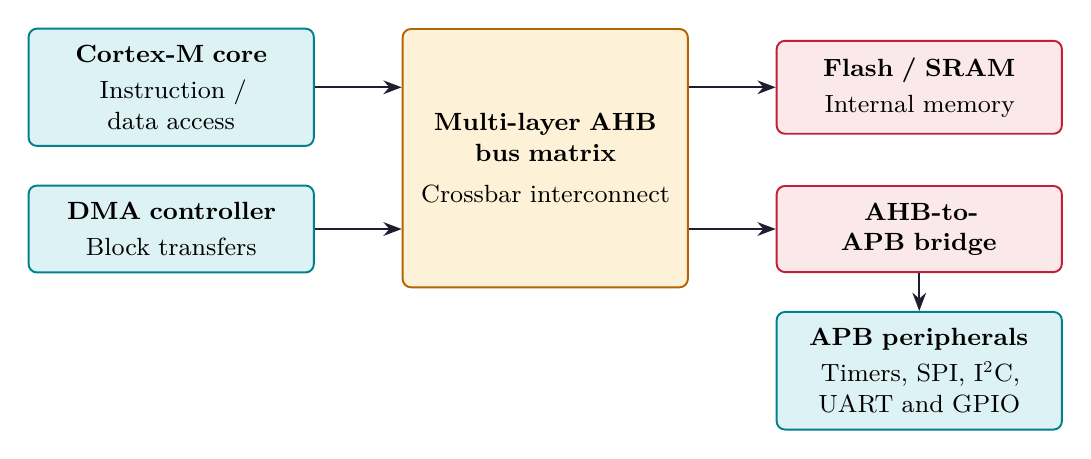
\begin{tikzpicture}[every node/.style={font=\small},
  unit/.style={align=center,text width=3.2cm,minimum height=1.08cm,inner sep=6pt}]
  \node[block,unit] (core) at (0,1.25) {\textbf{Cortex-M core}\\[2pt] Instruction / data access};
  \node[block,unit] (dma) at (0,-0.55) {\textbf{DMA controller}\\[2pt] Block transfers};
  \node[amberblock,unit,minimum height=3.28cm] (matrix) at (4.75,0.35)
    {\textbf{Multi-layer AHB}\\ \textbf{bus matrix}\\[4pt] Crossbar interconnect};
  \node[redblock,unit] (mem) at (9.5,1.25) {\textbf{Flash / SRAM}\\[2pt] Internal memory};
  \node[redblock,unit] (bridge) at (9.5,-0.55) {\textbf{AHB-to-APB bridge}};
  \node[block,unit] (peripherals) at (9.5,-2.35)
    {\textbf{APB peripherals}\\[2pt] Timers, SPI, I$^2$C,\\ UART and GPIO};
  \draw[arrow,thick] (core.east) -- (core.east -| matrix.west);
  \draw[arrow,thick] (dma.east) -- (dma.east -| matrix.west);
  \draw[arrow,thick] (mem.west -| matrix.east) -- (mem.west);
  \draw[arrow,thick] (bridge.west -| matrix.east) -- (bridge.west);
  \draw[arrow,thick] (bridge.south) -- (peripherals.north);
\end{tikzpicture}
\end{tcolorbox}

\subsection{GPIO Architecture and Configuration Modes}
Each GPIO pin on modern ARM MCUs (e.g., STM32) can be independently programmed via memory-mapped control registers into several electrical modes:
\begin{enumerate}[leftmargin=*]
  \item \textbf{Input Modes:}
  \begin{itemize}[leftmargin=*]
    \item \textit{Input Floating:} High-impedance input without pull resistors; used when external circuits drive both rails.
    \item \textit{Input Pull-Up / Pull-Down:} Connects weak internal resistor ($\approx 40\,\mathrm{k}\Omega$) to $V_{DD}$ or $\mathrm{GND}$ to prevent floating logic states.
    \item \textit{Analog Mode:} Disables the digital input Schmitt trigger to route pristine analog signals to the on-chip ADC.
  \end{itemize}
  \item \textbf{Output Modes:}
  \begin{itemize}[leftmargin=*]
    \item \textit{Push-Pull Output:} Active driving MOSFETs connect to $V_{DD}$ for logic high and $\mathrm{GND}$ for logic low. High drive strength ($\le 20\,\mathrm{mA}$).
    \item \textit{Open-Drain Output:} Only the pull-down N-MOSFET is active; logic high is high-impedance. Requires an external pull-up resistor. Essential for wired-AND buses like $\mathrm{I^2C}$.
  \end{itemize}
  \item \textbf{Atomic Bit Set/Reset Register (BSRR):}
  Writing a 1 to bits $0-15$ sets corresponding output pins; writing a 1 to bits $16-31$ resets them. Allows modifying single I/O pins in a single atomic bus cycle without dangerous software read-modify-write sequences on `ODR`.
\end{enumerate}

\subsection{Peripheral Interfacing: PWM, SPI, I2C, and UART}
\par\vspace{6pt}\noindent
\begingroup
\setlength{\extrarowheight}{2.5pt}
\begingroup
\setlength{\LTleft}{0pt}
\setlength{\LTright}{0pt}
\begin{longtable}{|B{2.4cm}|B{3.8cm}|>{\small\raggedright\arraybackslash}m{\dimexpr(\linewidth-2.4cm-3.8cm-6\tabcolsep-4\arrayrulewidth)/1\relax}|}
\hline
\textbf{Peripheral} & \textbf{Key Registers / Equations} & \textbf{Interfacing Mechanism and Practical Role} \\ \hline
\endfirsthead
\hline
\textbf{Peripheral} & \textbf{Key Registers / Equations} & \textbf{Interfacing Mechanism and Practical Role} \\ \hline
\endhead
Timer \& PWM & $f_{\mathrm{PWM}} = f_{\mathrm{TIM}}/D$\newline $D = (PSC+1)(ARR+1)$\par\smallskip $\text{Duty} \approx \frac{CCR}{ARR}\times 100\%$ & Prescaler ($PSC$) divides master clock; Auto-Reload ($ARR$) sets period; Capture/Compare ($CCR$) sets duty cycle. Drives DC motors, LED dimming, servos. \\ \hline
SPI Bus & $SCLK, MOSI$\newline $MISO, \overline{CS}$\newline Modes 0--3 ($CPOL, CPHA$) & High-speed full-duplex synchronous serial bus ($20+\,\mathrm{Mbps}$). Interfaced with SD cards, graphical LCDs, and precision sensors. \\ \hline
$\mathrm{I^2C}$ Bus & $SDA, SCL$ (Open-Drain) \newline Pull-ups ($4.7\,\mathrm{k}\Omega$) & Two-wire multi-master bus with 7-bit device addressing and ACK/NACK verification ($100\,\mathrm{kHz}$ standard, $400\,\mathrm{kHz}$ fast). Interfaced with EEPROMs, RTCs, temp sensors. \\ \hline
UART & Baud Generator, `TDR`, `RDR`, Status: $TXE, RXNE$ & Asynchronous point-to-point serial communication to PCs, GPS modules, and Bluetooth transceivers via FTDI/MAX232 chips. \\ \hline
\end{longtable}
\endgroup\par
\endgroup

\begin{tcolorbox}[tikzbox, title={ARM Timer PWM Generation via Auto-Reload ($ARR$) and Compare ($CCR$)}]
\centering
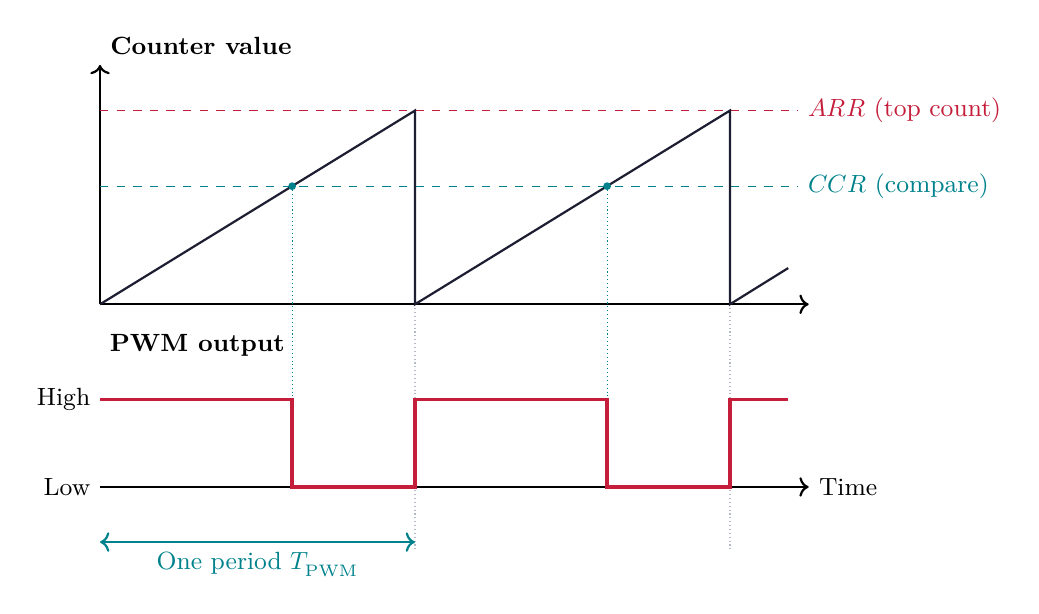
\begin{tikzpicture}[every node/.style={font=\small}]
  \draw[->,thick] (0,0) -- (9,0);
  \draw[->,thick] (0,0) -- (0,3.04)
    node[above,anchor=south west,font=\small\bfseries] {Counter value};
  \draw[dashed,myred] (0,2.46) -- (8.87,2.46) node[right] {$ARR$ (top count)};
  \draw[dashed,myteal] (0,1.5) -- (8.87,1.5) node[right] {$CCR$ (compare)};
  \foreach \compare in {2.44,6.44}
    \draw[densely dotted,myteal] (\compare,1.5) -- (\compare,-2.32);
  \foreach \reload in {4,8}
    \draw[densely dotted,mgframe] (\reload,0) -- (\reload,-3.14);
  \draw[thick,mydark] (0,0) -- (4,2.46) -- (4,0) -- (8,2.46) -- (8,0) -- (8.74,0.46);
  \fill[myteal] (2.44,1.5) circle[radius=1.4pt] (6.44,1.5) circle[radius=1.4pt];

  \node[above,anchor=south west,font=\small\bfseries] at (0,-0.78) {PWM output};
  \draw[->,thick] (0,-2.32) -- (9,-2.32) node[right] {Time};
  \node[left] at (0,-1.21) {High};
  \node[left] at (0,-2.32) {Low};
  \draw[very thick,myred] (0,-1.21) -- (2.44,-1.21) -- (2.44,-2.32)
    -- (4,-2.32) -- (4,-1.21) -- (6.44,-1.21) -- (6.44,-2.32)
    -- (8,-2.32) -- (8,-1.21) -- (8.74,-1.21);
  \draw[<->,thick,myteal] (0,-3.02) --
    node[below] {One period $T_{\mathrm{PWM}}$} (4,-3.02);
\end{tikzpicture}
\end{tcolorbox}

\begin{tcolorbox}[examplebox, title={Worked Interface Design: ARM Push-Button, PWM LED and SPI Sensor}]
\textbf{Design Scenario:} An STM32 microcontroller senses temperature via an SPI sensor, brightens an LED via Timer PWM, and toggles operation via an external push-button interrupt.
\par\vspace{4pt}
\begin{enumerate}[leftmargin=*]
  \item \textbf{Clock Enable:} Write to `RCC->APB2ENR` to enable clock gates for `GPIOA`, `GPIOB`, `AFIO`, and `TIM1`.
  \item \textbf{Button Input with EXTI:} Connect button to \texttt{PA0}. Configure \texttt{PA0} as Input with internal Pull-Up. Map \texttt{EXTI0} line to Port A via \texttt{AFIO->EXTICR[0]}. Unmask \texttt{EXTI0} in \texttt{EXTI->IMR}, configure falling-edge trigger in \texttt{EXTI->FTSR}, and enable \texttt{EXTI0\_IRQn} in the NVIC using \texttt{NVIC\_EnableIRQ(EXTI0\_IRQn)}.
  \item \textbf{PWM Output Configuration:} Configure \texttt{PA8} as Alternate Function Push-Pull (\texttt{TIM1\_CH1}). Set \texttt{TIM1->PSC = 71} (divide $72\,\mathrm{MHz}$ clock to $1\,\mathrm{MHz}$), set \texttt{TIM1->ARR = 999} ($1\,\mathrm{kHz}$ PWM frequency), and set \texttt{TIM1->CCR1 = 250} ($25\%$ duty cycle). Enable timer output via \texttt{TIM1->BDTR} and start timer counter via \texttt{TIM1->CR1}.
  \item \textbf{SPI Temperature Sensor Interfacing:} Configure \texttt{PB13} (SCK), \texttt{PB14} (MISO), and \texttt{PB15} (MOSI) as Alternate Function pins; configure \texttt{PB12} as general GPIO output for Chip Select ($\overline{\mathrm{CS}}$). To read: lower $\overline{\mathrm{CS}}$, write command byte into \texttt{SPI2->DR}, wait until \texttt{SPI\_SR\_TXE} and \texttt{SPI\_SR\_RXNE} set, read \texttt{SPI2->DR}, and raise $\overline{\mathrm{CS}}$.
\end{enumerate}
\end{tcolorbox}

\begingroup
\par\smallskip\noindent \textbf{ARM Architectural Features and Interfaces at a Glance}\par\nobreak
\par\vspace{5pt}
\begingroup
\setlength{\extrarowheight}{2.5pt}
\begingroup
\setlength{\LTleft}{0pt}
\setlength{\LTright}{0pt}
\begin{longtable}{|B{3.2cm}|>{\small\raggedright\arraybackslash}m{\dimexpr(\linewidth-3.2cm-6\tabcolsep-4\arrayrulewidth)/2\relax}|>{\small\raggedright\arraybackslash}m{\dimexpr(\linewidth-3.2cm-6\tabcolsep-4\arrayrulewidth)/2\relax}|}
\hline
\textbf{Feature / Interface} & \textbf{Architectural Function} & \textbf{Key Advantages and Properties} \\ \hline
\endfirsthead
\hline
\textbf{Feature / Interface} & \textbf{Architectural Function} & \textbf{Key Advantages and Properties} \\ \hline
\endhead
Load/Store Architecture & Decouples memory access from ALU & High compiler optimization, uniform single-cycle ALU execution. \\ \hline
Barrel Shifter & Inline operand shifting in ALU & Shifts operands (LSL, LSR, ASR, ROR) in zero extra clock cycles. \\ \hline
Conditional Execution & 4-bit condition field in instructions & Eliminates branch penalties and pipeline flushes in `if-else` blocks. \\ \hline
NVIC Controller & Integrated interrupt controller & Tail-chaining (6 cycles), automatic hardware stacking, low latency. \\ \hline
BSRR Register & Atomic GPIO bit manipulation & Fast, thread-safe bit set/reset without read-modify-write hazards. \\ \hline
Timer PWM & Hardware waveform generation & $PSC, ARR, CCR$ provide precision variable duty cycle with zero CPU overhead. \\ \hline
\end{longtable}
\endgroup\par
\endgroup
\endgroup

\newpage
% ─── Quick Revision Section ────────────────────────────────────────────────────
\begin{center}
  {\large\bfseries\color{myred} Quick Revision --- Module 4}\\[3pt]
  {\small\color{mydark} RISC Processors and ARM Interface Design $|$ EC403}
\end{center}
\noindent{\color{myred}\rule{\linewidth}{1.2pt}}\vspace{4pt}

\begin{tcolorbox}[formulabox, title={Key Formulas at a Glance}]
\renewcommand{\arraystretch}{1.3}
\noindent\begin{tabularx}{\linewidth}{B{4.5cm}Y}
Pipeline Speedup & $\mathbf{S_k} = \frac{n \times k}{k + n - 1} \xrightarrow{n \to \infty} k$ (for $k$-stage pipeline, $n$ instructions). \\
PWM Frequency & $f_{\mathrm{PWM}} = \frac{f_{\mathrm{TIM}}}{(PSC + 1) \times (ARR + 1)}$. \\
PWM Duty Cycle & $\text{Duty Cycle} = \frac{CCR}{ARR} \times 100\%$. \\
SPI Clock Frequency & $f_{\mathrm{SPI}} = \frac{f_{\mathrm{PCLK}}}{\text{Baud Prescaler}}$ (where Prescaler $\in \{2, 4, 8, \dots, 256\}$). \\
ARM PC Pipeline Offset & $\text{Actual Executing PC} = \text{Read PC} - 8$ (in 32-bit ARM state due to 3-stage pipeline). \\
\end{tabularx}\par
\end{tcolorbox}

\begin{tcolorbox}[defbox, title={One-Line Definitions}]
\begin{itemize}[leftmargin=*, itemsep=2.5pt]
  \item \textbf{Load/Store Architecture:} A RISC design principle where memory access is strictly confined to `LDR` and `STR` instructions, with all arithmetic performed between registers.
  \item \textbf{Operand Forwarding:} A hardware pipeline technique that feeds an ALU result directly from a pipeline stage register to a subsequent instruction, eliminating data dependency stalls.
  \item \textbf{RAW Hazard (True Dependency):} A pipeline hazard occurring when an instruction attempts to read a register before an immediately preceding instruction writes to it.
  \item \textbf{Barrel Shifter:} An on-chip hardware shifter in ARM that performs bit shifting on the second operand in zero extra clock cycles as part of an ALU operation.
  \item \textbf{Tail-Chaining (NVIC):} An ARM interrupt optimization that switches directly between back-to-back pending interrupts in 6 cycles without redundant register popping and pushing.
  \item \textbf{BSRR (Bit Set/Reset Register):} A 32-bit GPIO register in ARM microcontrollers enabling atomic single-cycle setting and clearing of port pins without read-modify-write hazards.
  \item \textbf{Push-Pull Output:} An active GPIO driving configuration using complementary transistors to actively source current to $V_{DD}$ or sink current to $\mathrm{GND}$.
  \item \textbf{Open-Drain Output:} A GPIO output mode where the transistor only sinks current to ground, requiring an external pull-up resistor to pull the line high.
\end{itemize}
\end{tcolorbox}

\begin{tcolorbox}[exambox, title={Frequently Asked / Viva Questions}]
\begin{enumerate}[leftmargin=*, label=\textbf{Q\arabic*.}, itemsep=2.5pt]
  \item \Q{What are the primary differences between RISC and CISC architectures?}
  RISC uses uniform 32-bit instructions, load/store architecture, single-cycle execution, large register files, and hardwired control; CISC uses variable-length instructions, complex memory addressing, multi-cycle execution, and microprogrammed control.
  \item \Q{Name the stages in a classic 5-stage RISC pipeline.}
  Instruction Fetch (IF), Instruction Decode \& Register Read (ID), Execute / Address Calculation (EX), Memory Access (MEM), and Write Back (WB).
  \item \Q{How does operand forwarding resolve RAW data hazards?}
  It routes the computed result directly from the output of the EX/MEM or MEM/WB pipeline stage registers back into the ALU input multiplexer before it is written to the register file.
  \item \Q{What does the mnemonic ARM7TDMI stand for?}
  ARM7 core with: \textbf{T} = Thumb 16-bit instruction set; \textbf{D} = JTAG On-chip Debug; \textbf{M} = 32-bit Fast Multiplier; \textbf{I} = EmbeddedICE in-circuit emulation logic.
  \item \Q{What are the main advantages of the ARM Cortex-M NVIC?}
  It provides ultra-low deterministic interrupt latency (12 cycles), automatic hardware register stacking, tail-chaining (6 cycles), and late-arriving interrupt preemption.
  \item \Q{Why does the ARM core include an on-chip Barrel Shifter?}
  It allows one operand to be shifted or rotated by arbitrary bits concurrently during an ALU operation in a single clock cycle without any execution time penalty.
  \item \Q{Explain the conditional execution feature of 32-bit ARM instructions.}
  Every 32-bit instruction contains a 4-bit condition field; the instruction executes only if the condition flags ($N, Z, C, V$) match, avoiding branch instructions in small conditional statements.
  \item \Q{What is the difference between MSP and PSP in ARM Cortex-M?}
  Main Stack Pointer (MSP) is used by the OS kernel and exception/interrupt handlers; Process Stack Pointer (PSP) is used by user application threads in an RTOS environment.
  \item \Q{Why is atomic bit manipulation via BSRR preferred over modifying ODR in GPIO?}
  BSRR sets or resets pins in a single write operation, preventing race conditions and corrupted pins caused by read-modify-write operations when interrupts occur.
  \item \Q{How are PWM duty cycle, SPI, and I2C buses interfaced in ARM microcontrollers?}
  PWM duty cycle is adjusted via the Capture/Compare Register ($CCR/ARR \times 100\%$); SPI uses 4 modes determined by $\mathrm{CPOL}$ and $\mathrm{CPHA}$; $\mathrm{I^2C}$ uses open-drain outputs with pull-up resistors to prevent contention.
\end{enumerate}
\end{tcolorbox}

\end{document}
